\chapter{Dispersion relation}
\label{disperrel}
A dispersion relation relates the wavenumber of a wave to its frequency. We
will see that this relation is of utmost importance when discussing periodic
lattices as only waves of certain frequencies are transmitted by the lattice.

\section{1d lattice}
\begin{center}
  \begin{tikzpicture}
  {[start chain,every on chain/.style=join,every join/.style=-,
    state/.style={circle,draw,minimum size=1.5cm}]
     \node[on chain] (A) {$\cdots$};
     \node[on chain,state] (B) {$M_{n-1}$};
     \node[on chain,state] (C) {$M_n$};
     \node[on chain,state] (D) {$M_{n+1}$};
     \node[on chain] (E) {$\cdots$};
  }
  \end{tikzpicture}
\end{center}
Let us start our discussion with the most basic one-dimensional case. In this
case, we have masses of equal mass, $m$ spread out evenly across one dimension.
All neighbouring masses are connected by an elastic force which scales
proportionally with distance, i.e. $F = kx$ for some $k$.

% TODO: Add discussion about transverse waves into appendix?
\textit{Note}: It is very useful to think of this system as a mass-spring
system. For simplicity, we will be considering longitudinal waves, however the
same analysis can be done for transverse waves as we show in the appendix.

With this one-dimensional case set up, we now want to find out what forms of
waves it allows to propagate. We do this by considering only nearest neighbour
interactions and examining the elementary unit of the lattice which can be
repeated by translation to form the full lattice.

So let us consider three masses side-by-side in our lattice, $M_{n-1}$, $M_n$
and $M_{n+1}$ which are $y_{n-1}$, $y_n$ and $y_{n+1}$ displacement away from
their equilibrium positions. By focusing on the centre mass and considering
only nearest neighbour interactions, by Hooke's Law, we have that the force on
$M_n$

\begin{align}
  F_{n}=\sum F=k\left(y_{n-1}+y_{n+1}-2y_{n}\right) \label{eq:HL}
\end{align}

At the same time, we have by Newton's 2nd Law that

\begin{align}
  F_{n}=m\frac{d^{2}}{dt^{2}}y_{n}
\end{align}

Taking $y_n$ to be the general wave solution

\begin{align}
  &y_{n}=\hat{y}_{n}e^{-i\Omega t} \\
  \Rightarrow &\frac{d^{2}}{dt^{2}}y_{n}=-\Omega^{2}y_{n} \\
  \Rightarrow &F_{n}=-m\Omega^{2}y_{n}a \label{eq:N2L}
\end{align}

where $\Omega$ is the frequency of the wave and $\hat{y}_{n}$ is the complex
amplitude.

Therefore, we have by \eqref{eq:HL} and \eqref{eq:N2L} that

\begin{align}
  &-m\Omega^{2}y_{n}=k\left(y_{n-1}+y_{n+1}-2y_{n}\right) \\
  \Rightarrow &\left(-\frac{m}{k}\Omega^{2}+2\right)y_{n}-y_{n-1}-y_{n+1}=0
    \label{eq:HLN2L}
\end{align}

Now since we have that $M_{n-1}$ and $M_{n+1}$ are equidistant from $M_{n}$ at
equilibrium (i.e. the lattice is periodic), we can describe the phase shift in
the wave solution as

\begin{align}
  y_{n-1}=e^{-i\kappa}y_n,\ \ y_{n+1}=e^{i\kappa}y_n
\end{align}

Hence, from \eqref{eq:HLN2L}, we see that

\begin{align}
  &\left(-\frac{m}{k}\Omega^{2}+2-e^{-i\kappa}-e^{i\kappa}\right)y_{n}=0 \\
  \Rightarrow &\cos\left(\kappa\right)=-\frac{m}{2k}\Omega^{2}+1
\end{align}

Therefore, we now have an equation linking the wave number $\kappa$ and the
frequency $\Omega$ of waves propagating across our 1d lattice. By initialising
$m$ and $k$ we can use this equation to plot the dispersion curve of our
system. By setting $m=k=1$, we get the dispersion curve in Figure
~\ref{fig:dc1}.

\begin{figure}[!h]
\centering
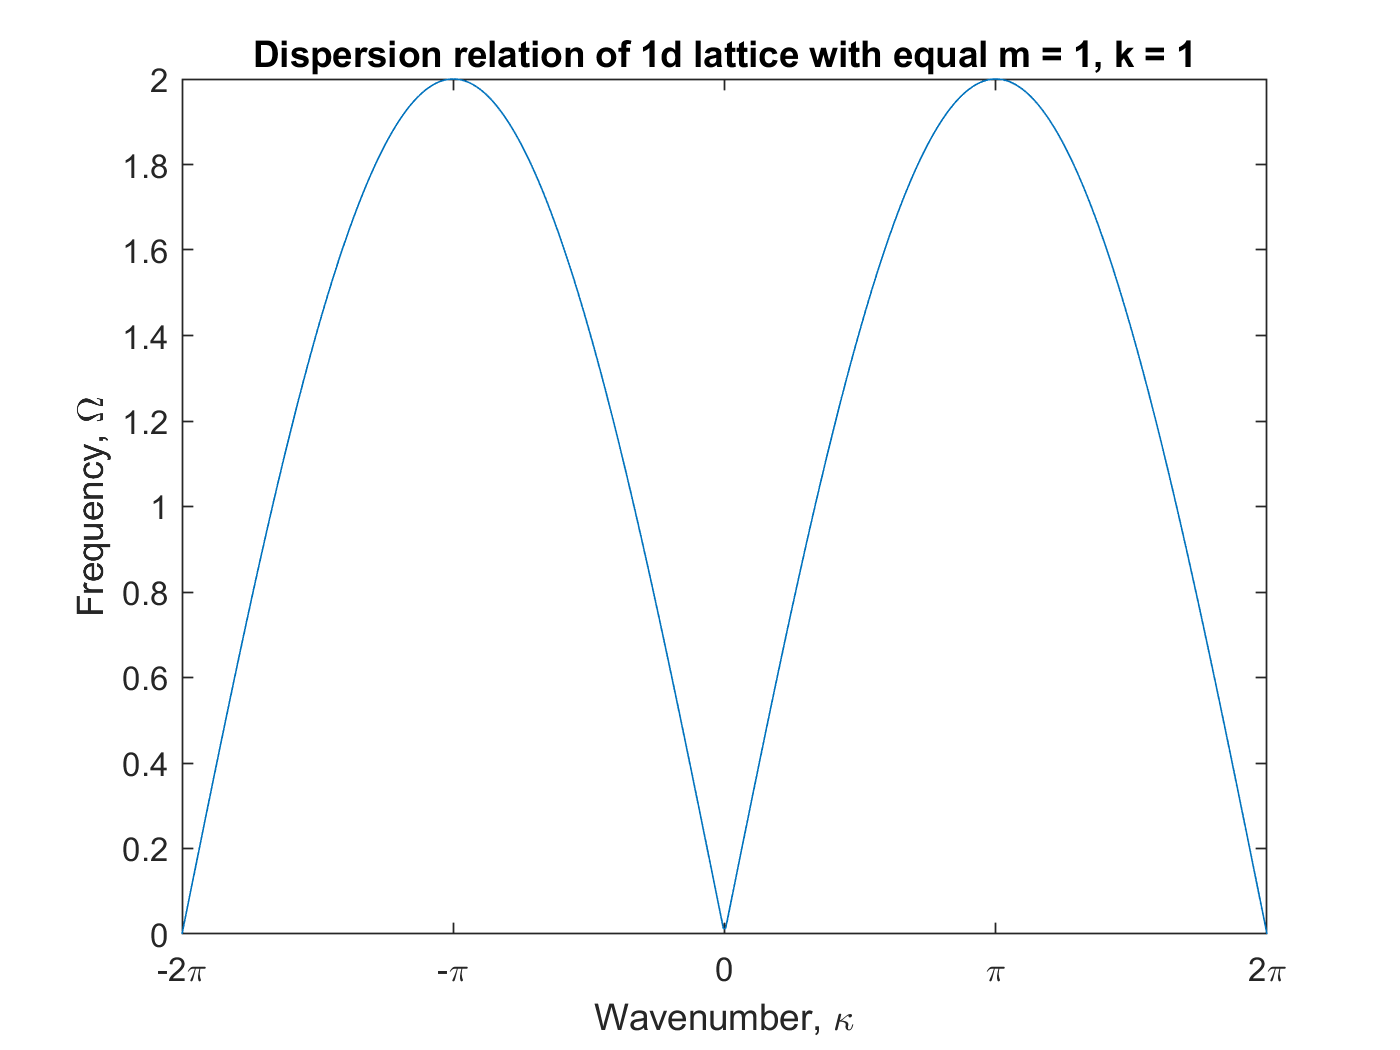
\includegraphics[width=0.8\textwidth]{imgs/1ddispersion.png}
\caption{\label{fig:dc1}Dispersion relation of a 1d monoatomic
         chain.}
\end{figure}

The first interesting thing to notice about this dispersion relation is that
the curve seems to be periodically repeating. More precisely, if we look at the
curve between $-\pi$ and $\pi$, we can see that translating this portion of the
graph left or right by $2\pi$ will give us the rest of the dispersion relation.
This range of wave numbers is known as the first Brillouin zone, which we will
discuss more in the context of 2d lattices in Chapter \ref{brizones}.

\section{2d square lattice}
\begin{center}
  \begin{tikzpicture}
{[start chain,every node/.style={circle,draw},every join/.style=-]
\foreach \X in {-2,2,...,-2}
{\foreach \Y in {-2,2,...,-2} 
  {[start chain]
   \node[on chain,join] at (\X+1,\Y+1) {$M_{1}$};
   \node[on chain,join] at (\X+1,\Y-1) {$M_{2}$};
   \node[on chain,join] at (\X-1,\Y-1) {$M_{3}$};
   \node[on chain] at (\X-1,\Y+1) {$M_{4}$};}}}
  \end{tikzpicture}
\end{center}

We now extend this analysis to an infinite two-dimensional square lattice. Each
elementary square cell contains four masses $M_i$ for $i\in\left[1, 4\right]$
which are arranged clockwise from the top right. We take $n$ and $m$ to be the
vertical and horizonal directions respectively, so that relative to cell $(n,
m)$ we have cell $(n+1,m)$ above and cell $(n,m+1)$ to the right. With this
setup, we can now label each mass uniquely, e.g. $M_i$ in cell $(n, m)$ is
labelled $M_i^{n,m}$.

Each mass is elastically connected to its direct neighbours, e.g. $M_1^{n,m}$
is connected to $M_2^{n,m}$, $M_4^{m,n}$, $M_2^{n,m+1}$ and $M_4^{n+1,m}$. We
have the spring constant $k$ between masses in the same cell and $\tilde{k}$
between masses in adjacent cells.

Now again we consider only nearest neighbour interactions. Focusing on the
elementary cell $(n,m)$ and its adjacent cells, using Hooke's law and Newton's
2nd law on each of the masses in cell $(n,m)$, we see that we can form four
coupled second order differential equations.
%TODO: Complete discussion of square lattice

\subsection{Brillouin zones}
\label{brizones}
The concept of Brillouin zones was first defined by Leon Brillouin in his book
on wave propagation in periodic structures.\cite{brillouin}
%TODO: Complete discussion of brillouin zones

\section{2d hexagonal lattice}
We will now consider how waves propagate across a 2d lattice made of hexagonal elementary cells. 

%TODO: Add image to show model
Consider an infinite 2d plane made of hexagonal unit cells of six masses $M_i$
for $i\in\left[1,6\right]$, which are arranged in an inner hexagon rotated
$\frac{\pi}{6}$ relative to each cell. Now we take the spring constant to be $k$
between masses within the same cell and $\tilde{k}$ between masses in adjacent
cells.
%TODO: Complete discussion of hexagonal lattice

